\vspace{-8mm}
\section{Introduction}
Suicide is responsible for 1·5\% of global mortality and is one of the most challenging public mental health 
issues \cite{oconnor_psychology_2014}.
Suicidality includes any thoughts or actions by an individual that could %have resulted 
result in death \cite{turecki_suicide_2016}. 
Preventing death by suicide is a priority for health care services internationally \cite{zalsman_suicide_2016}, but poses a great challenge since accurately predicting an episode of suicidality is almost impossible\cite{mchugh2019,velupillai_risk_2019}. Furthermore, many deaths by suicide occur in people who did not have a known diagnosed mental health condition when they died\cite{stone_vital_2018}. Our ability to understand suicide has therefore been hampered by our ability to obtain data ``in situ''~\cite{nock2019}.
Platforms such as Reddit and Twitter are starting to offer a new and uniquely transparent window into suicide and other mental health issues. Unlike traditional health records, social media posts are authored by the users themselves. Also, in contrast to formal clinical settings, users on such platforms express themselves freely rather than regulating answers to establish a positive impression or be socially desirable \cite{van_de_mortel_role_2008}, thus providing a fresh and honest perspective~\cite{gkotsis2017characterisation}. Social media have therefore become a fertile ground for mental health studies, leading to new results in %depression\cite{}, anxiety~\cite{}, autism, addiction, dementia and other problems~\cite{de2014mental,park2018examining,shen2017detecting,park2017longitudinal,DeChoudhury2016,DeChoudhury2014}.
depression, anxiety, autism, and other problems~\cite{de2014mental,park2018examining,shen2017detecting,park2017longitudinal,DeChoudhury2016,DeChoudhury2014}.
 
Recent studies have shown promising results in modeling and measuring signals and patterns in Reddit communities related to mental health. For instance, statistical relations of mental health and depression communities with suicide ideation have been studied \cite{DeChoudhury2014,DeChoudhury2016}. The authors explored linguistic and social characteristics that evaluate users' propensity to suicidal ideation. Approaches to classify reddit posts as related to certain mental health conditions have also been successfully developed, showing that there are certain characteristics specific to mental health-related topics in posts that can be automatically captured\cite{gkotsis2017characterisation}. Furthermore, in a study focused on reddit posts related to anxiety, depression and post-traumatic stress disorder, the authors show that these online communities exhibit themes of a supportive nature, e.g. gratitude for receiving emotional support\cite{park2018examining}. Positive effects of  participation in such fora have also been shown by improvements in members' written communication\cite{info:doi/10.2196/jmir.8219}. The supportive nature of comments in the SuicideWatch forum has also been studied by automatic identification and classification of helpful comments with promising results\cite{Kavuluru:2016:CHC:2975167.2975170}.
Naturally, several studies that have been based on these types of online communities 
look at the \emph{textual} content of these online fora and produce inferences about psychological states. In our work, we conjecture that apart from textual metrics, it is important to quantify the differences in the \emph{structure} of a supportive conversation.



In the context of suicide, social media occupies an important ``clinical whitespace''~\cite{coppersmith2018} --  long intervals between clinical encounters that are filled with frequent posts on social media. These provide the potential for increased visibility into patient mental states. Studies have started to use social media posts both to understand population level responses to external triggers such as celebrity suicides~\cite{kumardetecting,karamshuk} and as a means to assess suicide risk~\cite{shing2018,clpsych}.   

While these are important first steps, such studies 
%such as these 
could be affected by the very nature of social media: it is unregulated, and problems such as cyberbullying\cite{luxton2012social,patton2014social} could potentially affect the variables being studied.  For instance, risk of suicide may be exacerbated just by participating on online social platforms. Therefore, we believe it is crucial to understand first the \emph{nature} of the conversations that happen online around suicide and suicidal behaviour. This paper aims to answer the question:  Does social media activity provide a supportive medium for potentially vulnerable patients? We address this  by studying the interactions of users on  \textbf{SuicideWatch}(\url{https://www.reddit.com/r/SuicideWatch/}), an online community (``subreddit'') on the social media platform Reddit. SuicideWatch is a heavily moderated forum, keeping messages and conversations on topic, and is  focussed solely on the topic of suicide. 
The moderators take the message of peer support seriously, and are governed by guidelines that prohibits false promises, abuse, tough love and other clinically concerning methods of conversations~\cite{BBC_suicidewatch}
It has therefore been the focus of recent research~\cite{shing2018} and shared tasks which aim to advance the state of the art~\cite{clpsych}. 

In contrast with previous studies which only looked at original posts on SuicideWatch, we look at the entire conversation ``thread''. In other words, we start with the content from the Original Poster (OP), but we also include the hierarchically nested thread of replies to the original post, the replies to those replies, and so on.
%
%Online communities, or fora, offer a platform for users to directly interact with each other. Reddit\footnote{\url{http://reddit.com/}} is one of the largest online communities which contains a number of sub-communities (so called \emph{subreddits}) that can deal with myriad of topics. On this platform, several sub-reddits are specifically tailored to mental health-related topics, such as \emph{depression}, \emph{anxiety} or \emph{alcoholism}. There are thousands of users on these communities, exchanging thoughts and asking for help. These forums offer a unique opportunity to study the way people describe or discuss their problems in their own voice. 
Further, most previous studies have aimed at studying the \emph{content} of posts and their characteristics in relation to other posts. But an important aspect of online communities is their supportive \emph{function}, where users can turn to these platforms not only to express their thoughts and concerns, but also to receive support from the community. This support often manifests as an emergent conversation between many users and the one in distress. Hence here we propose a framework that captures the structure of a conversation thread and develop metrics that capture the \emph{macroscopic} properties of a conversation that involve the entire thread and the users participating in it as well as \emph{mesocopic} properties of a conversation that involve the immediate interactions with the one in distress. 

\begin{table}
	\resizebox{0.5\linewidth}{!}{
		\begin{tabular}{l|p{8cm}}
			\textbf{Terminology} & \textbf{stands for}\\
			$RP$   & Root post which begins a new thread on a subreddit \\
			$OP$  & Original poster who posts the Root post for a thread \\
			$SW$ & The suicide watch Subreddit \\
			$FP$  & Front page of Reddit. \\
		\end{tabular}}
	\caption{Notations and Terms.}
    \label{notations}
\end{table}

To model the conversation structure, we represent conversations in a forum using two graph-based abstractions: \textit{User interaction graphs}, which model the user-to-user exchange of messages, and  \textit{reply graphs}, which capture the structure of the dialogue on the forum, see example in Figure \ref{Fig:GraphExamples}. The complete processing pipeline can be seen in Figure~\ref{fig:pipeline}. We describe the pipeline and the metrics in detail in the \nameref{section:methods} section.
We then propose metrics that quantify the macroscopic structure of the two graphs we construct:
\textbf{Responsiveness} measures how quickly the responses accumulate in the reply graph ; \textbf{Centrality} of the OP] measures how important the OP is to the conversation thread by computing the betweeness centrality\cite{white1994betweenness} of the OP in the user graph; \textbf{Reciprocity} measures the extent to which users obtain replies when they post something, by computing the fraction of edges in the user graph that are bidirectional.;\textbf{Branching factor} measures how the reply graph fans out, i.e., the number of replies a post obtains. 
% \begin{description}
% \item[Responsiveness] measures how quickly the responses accumulate in the reply graph
% \item[Centrality of the OP] measures how important the OP is to the conversation thread by computing the betweeness centrality\cite{white1994betweenness} of the OP in the user graph
% \item[Reciprocity] measures the extent to which users obtain replies when they post something, by computing the fraction of edges in the user graph that are bidirectional.
% \item[Branching factor] measures how the reply graph fans out, i.e., the number of replies a post obtains. 
% \end{description}

To measure local or mesoscopic structure, we turn to network motifs~\cite{milo2002network}. We propose a new method to count and characterise local structures, called anchored triadic motifs. Triadic motifs traditionally consider three nodes at a time~\cite{milo2002network}. Given the primacy of the OP, our method distinguishes variants based on where the OP is situated in a triad, to understand how the local patterns of  communications support the OP.  
In summary, this paper makes four key contributions: 

\begin{figure*}[!h]
    \centering
    % \hspace*{-5mm}
    \subfloat[]{
        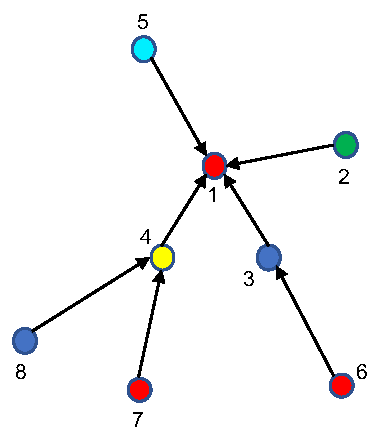
\includegraphics[width=0.2\textwidth ]{Figures/reply_graph.pdf}
        \label{fig:rGraphSW}
    }
\hspace{30mm}
    \subfloat[]{
        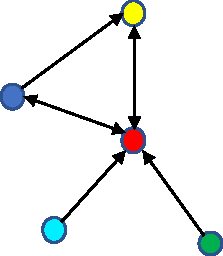
\includegraphics[width=0.2\textwidth]{Figures/user_graph.pdf}
        \label{fig:uGraphSW}
    }
    
    \caption{ Figure ~\ref{fig:rGraphSW} shows a sample reply graph constructed from a real thread in SW that contains 8 posts by 5 unique users. Each node represents a post and a directed edge is drawn from one node to another node when the first node is a reply to the second node. Thus, for example, Node 1 is the original post, with four replies (posts 2, 3, 4 and 5). Each node is given a colour based on the author of the post that the node represents, and each distinct colour represents a distinct author. Thus, from the reply graph, we can deduce that the original poster (Red node) obtained replies from the blue, green, yellow and purple users. In turn, the red node replied back to purple and yellow nodes ,but not to the blue and green nodes. The entire list of directed interactions is captured in a user interaction graph in Figure ~\ref{fig:uGraphSW}, where each coloured node represents the corresponding user who wrote a post on the thread, and the directed edges represent the replies.}
    \label{Fig:GraphExamples}
\end{figure*}

%In summary, this paper makes four key contributions: 
\setlist{nolistsep}
\begin{itemize}[noitemsep]
    \item We develop a framework  that abstracts out both the structure and semantics of a threaded conversation on the web
    \item Using this abstraction, we develop metrics which quantify the macroscopic (thread-wide) properties of conversations on SuicideWatch. 
    \item We develop a new method, which we term \textit{anchored triadic motifs}, to understand the mesoscopic or local structure of SuicideWatch conversations using triadic network motifs. Our method adapts triads by anchoring on the position of the Original Poster (OP), thereby distinguishing the OP from the other posters and helps understand how the conversation supports the OP's needs. 
    \item We show that there are significant statistical differences, both in the macroscopic and mesoscopic realm, that differentiate a SuicideWatch conversation from a generic conversation. 
\end{itemize}


